% ==========================================================================================
\section{How Lightning Nodes Upgrade}
\label{sec:dynamics}

\subsection{Adoption of new release lines}
Fig.~\ref{fig:linemix} shows the release-line mix of live LND and CLN nodes. Each new LND line displaces its
predecessor within a few months but leaves a tail: at the cutoff, \PctOldLndLive\% of live LND nodes were still on a
line older than 0.19, released in May~2025. New lines reached half of live LND nodes \TFiftyLndMin--\TFiftyLndMax{}
days after release (Fig.~\ref{fig:adoption}); half of live capacity moved as fast or faster for 0.18 and 0.19
(\TFiftyCapLndEighteen{} and \TFiftyCapLndNineteen{} days) but more slowly for 0.20 (\TFiftyCapLndTwenty{} days).
Counting the fleet as independent nodes would put LND 0.20 at 50\% of nodes after \TFiftyLndTwentyWithFleet{} days
instead of \TFiftyLndTwenty{}. CLN lines took \TFiftyClnMin--\TFiftyClnMax{} days. Every LND line from 0.18 on was
announced by a few nodes \FirstSeenLndMin--\FirstSeenLndMax{} days before its release: developers and early adopters
running unreleased builds on mainnet.

\begin{figure*}[t]
\centering
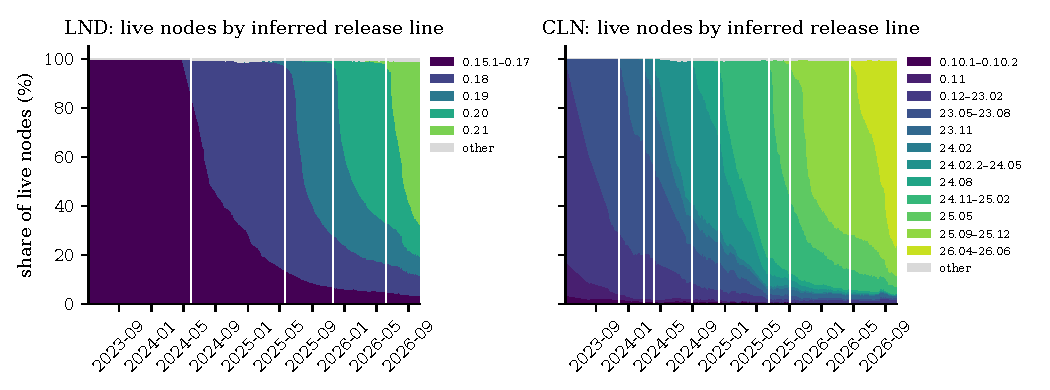
\includegraphics[width=\textwidth]{figures/fig1_line_mix.pdf}
\caption{Live LND and CLN nodes by inferred release line (likely line), excluding the managed fleet. White lines mark
releases. Lines under 2\% of nodes throughout are grouped as ``other''.}
\label{fig:linemix}
\end{figure*}

\begin{figure*}[t]
\centering
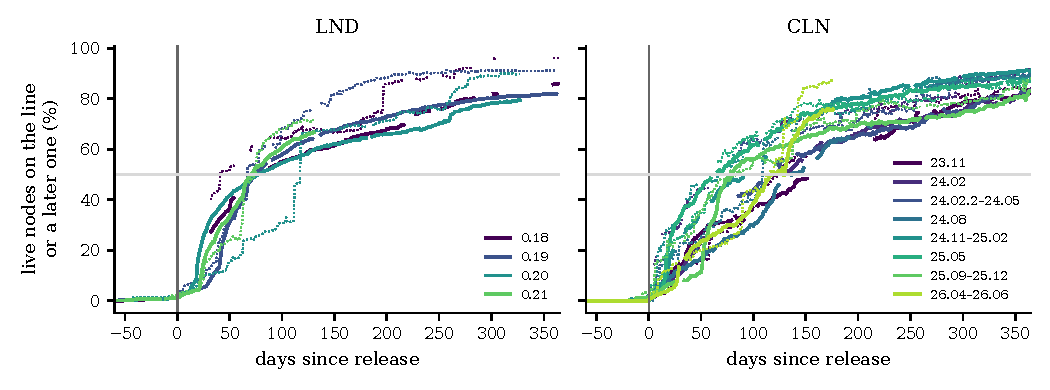
\includegraphics[width=\textwidth]{figures/fig3_adoption.pdf}
\caption{Share of live nodes (solid) and of their live capacity (dotted) on each release line or a later one, by
days since the line's release. Lines are broken across snapshot gaps longer than three days.}
\label{fig:adoption}
\end{figure*}

\subsection{Time to upgrade}
Adoption curves mix upgrades with nodes arriving and leaving. To follow operators, we take every node that is live
on an older line on the release day of LND 0.19, 0.20 or 0.21 or of a CLN line from 23.11 on, and measure the time
until it is first seen on the new line or a later one. Snapshot gaps leave the upgrade day inside an interval (for
\PctIntervalNarrow\% of LND upgrades it is at most two days wide); nodes that stop being live before upgrading are
censored at their last live day. The share upgraded by day $t$ is the nonparametric maximum-likelihood estimate for
interval-censored data~\cite{turnbull1976empirical}. Half of the LND nodes upgraded within \MedianLNDAll{} days and
\ByYearLNDAll\% within a year; for CLN the median is \MedianCLNAll{} days. Size matters at the bottom: the smallest
quarter of LND nodes by live capacity took a median \MedianLNDSmall{} days, the largest quarter \MedianLNDLarge{}
(Fig.~\ref{fig:ttu}).

Table~\ref{tab:hazard} fits a discrete-time model of the weekly probability of upgrading for LND. Larger nodes
upgrade sooner (odds ratio \ORCapacity{} per tenfold capacity, \ORChannels{} per tenfold channel count), and so do
Tor-only nodes (\ORTor{}), which make up most of the platform waves of \S\ref{sec:waves}. A node more than one line
behind when the release ships is far less likely to move (\ORBehind{}): the tail is made of nodes that skipped releases before.
Nodes with LND's default colour are no slower (\ORDefaultColor{}), and nodes seen before 2024 upgrade at the same
rate as newer ones (\OROld{}).

\begin{figure*}[t]
\centering
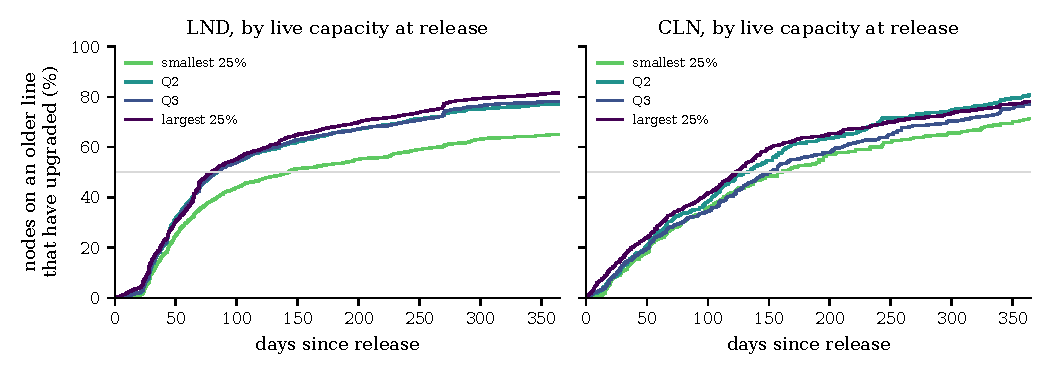
\includegraphics[width=\textwidth]{figures/fig4_time_to_upgrade.pdf}
\caption{Share of nodes that were live on an older line at a release and have since been seen on the new line or a
later one, by quartile of live capacity at the release (Turnbull estimate; LND 0.19--0.21, CLN 23.11--26.04).}
\label{fig:ttu}
\end{figure*}

\begin{table}[t]
\centering\small
\caption{What predicts upgrading: discrete-time logit on node-weeks after each LND release (week and release fixed effects; standard errors clustered by node). Odds ratios with 95\% CI.}
\label{tab:hazard}
\begin{tabular}{lrr}
\toprule
Covariate & Odds ratio & 95\% CI \\
\midrule
Capacity ($\times$10) & 1.11 & [1.07, 1.16] \\
Channels ($\times$10) & 1.15 & [1.06, 1.24] \\
Tor-only & 1.59 & [1.50, 1.69] \\
LND default colour & 1.08 & [1.03, 1.14] \\
Seen before 2024 & 1.01 & [0.96, 1.07] \\
$>$1 line behind & 0.19 & [0.18, 0.21] \\
\midrule
Nodes / node-weeks & \multicolumn{2}{r}{7,218 / 228,254} \\
\bottomrule
\end{tabular}
\end{table}

